\subsection*{Ebene Wellen (TEM)}
\begin{center}
\begin{tabular}{ccc} \toprule
Bezeichnung & Symbol & Einheit \\ \midrule
Wellenwiderstand & $Z_F$ & \si{\ohm} \\
Brewsterwinkel (nur parallel) & $\theta_B$ &  \\
Wellenzahl & k & \\
Eindringtiefe & $\delta$ & \si{\meter} \\
Poynting-Vektor & $\vec{S}$ & $\si{\watt\per\meter^2}$ \\
\bottomrule
\end{tabular}
\end{center}

\begin{align*}
Z_F &= \frac{\vec{E}}{\vec{H}} = \sqrt{\frac{\mu_0 \mu_r}{\epsilon_0 \epsilon_r}} = Z_{F0} \sqrt{\frac{\mu_r}{\epsilon_r}} \\
\lambda &= \frac{v_\text{ph}}{f} = \frac{\lambda_0}{\sqrt{\mu_r \epsilon_r}} \\
v_\text{ph} &= \frac{\omega}{\beta} = \frac{c_0}{\sqrt{\epsilon_r \mu_r}} = v_g \\
\beta &= \frac{\omega}{v_\text{ph}} = \frac{2 \pi}{\lambda}
\end{align*}

\begin{description}
\item[Allgemein]
\begin{align*}
\vec{E} &= \vec{E}_0 e^{-j\vec{k}\cdot \vec{r}} \\
\vec{H} &= \vec{H}_0 e^{-j\vec{k}\cdot \vec{r}} \\
\vec{k} &= k_x \vec{e}_x + k_y \vec{e}_y + k_z \vec{e}_z \\
\vec{r} &= x \vec{e}_x + y \vec{e}_y + z \vec{e}_z \\
\vec{k} \cdot \vec{k} &= \beta^2 - \alpha^2 -j2\vec{\alpha}\cdot \vec{\beta} = \omega^2 \epsilon \mu
\intertext{mit $\vec{\beta} = \vec{k}$ und $\vec{\alpha} = 0$}
\vec{E} &= \vec{E}_0 e^{-j\vec{k}\cdot \vec{r}} \\
\vec{H} &= \frac{1}{Z_F} \left( \vec{e}_k \times \vec{E}_0 \right) e^{-j \vec{k}\cdot \vec{r}} \\
\vec{k} &= k \vec{e}_k \\
k &= \omega \sqrt{\epsilon \mu} \\
\vec{S} &= \frac{\vec{e}_k}{2Z_F^*} \left( \vec{E} \cdot \vec{E}^* \right) = \frac{\vec{e}_k Z_F}{2} \left( \vec{H} \cdot \vec{H}^* \right)
\intertext{für $\vec{\beta} \cdot \vec{\alpha} = 0$ entstehen evaneszente Wellen}
\end{align*}

\item[Polarisation] Hängt vom $E$-Feld ab. Wenn $E_i < E_j$, dann elliptisch. Wenn $E_i = E_j$, dann zirkular. Wenn $E_i = 0$, dann linear. 

\item[Poynting-Vektor für zeitgemittelte Größen]
\begin{equation*}
\vec{S} = \frac{1}{2} \Re\left\{{\vec{E}\times \vec{H}}\right\}
\end{equation*}

\item[Strahlungsleistungsdichte]
\begin{equation*}
\vec{S} = \frac{1}{2} \frac{\vec{E}^2}{Z_{F}} = \frac{1}{2} \vec{H}^2 \cdot Z_F
\end{equation*}

\item[Brechungsgesetz] Krümmung erfolgt in Richtung des größeren $\epsilon_r$.

\begin{minipage}{0.52\linewidth}
	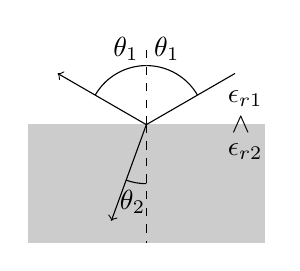
\begin{tikzpicture}[scale=1, every node/.style={scale=1}]
	\filldraw [color=black!20] (0,-0.5) rectangle(3,1);
\coordinate (center) at (1.5,1);
\draw (center) -- ++(30:1.3) ;
\draw [->] (center) -- ++(150:1.3);
\draw [dashed] (center) -- ++(0,1);
\draw [dashed] (center) -- ++(0,-1.5);

\draw (center) +(0,0.75)arc [radius=0.75,start angle=90, end angle=30];
\draw (center) +(0,0.75)arc [radius=0.75,start angle=90, end angle=150];

\path (center) ++(75:1) node{$\theta_1$};
\path (center) ++(105:1) node{$\theta_1$};

\draw [->] (center) -- ++(250:1.3);
\draw (center) +(0,-0.75)arc [radius=0.75,start angle=270, end angle=250];
\path (center) ++(260:1) node{$\theta_2$};

\path (center) ++(15:1.3) node{$\epsilon_{r1}$};
\path (center) ++(345:1.3) node{$\epsilon_{r2}$};
\path (center) ++(0:1.2) node{$\wedge$};
	\end{tikzpicture}
\end{minipage}
\begin{minipage}{0.47\linewidth}
\begin{equation*}
\sqrt{\frac{\epsilon_{r1}}{\epsilon_{r2}}} = \frac{\sin\theta_2}{\sin\theta_1}
\end{equation*}
\end{minipage}

\item[Brechzahl]
\begin{equation*}
n = \frac{c_0}{v_\text{ph}} = \sqrt{\epsilon_r\mu_r}
\end{equation*}

\item[Fresnel-Koeffizienten für schrägen Einfall auf dielektrische Grenzfläche] 
\begin{align*}
R_{||} &= \frac{\sqrt{\epsilon_{r2}} \cos{\theta_1} - \sqrt{\epsilon_{r1}} \cos{\theta_2}}{\sqrt{\epsilon_{r2}} \cos{\theta_1} + \sqrt{\epsilon_{r1}} \cos{\theta_2}} = \frac{Z_{F1} \cos{\theta_1} - Z_{F2} \cos{\theta_2}}{Z_{F1} \cos{\theta_1} + Z_{F2} \cos{\theta_2}} \\
T_{||} &= \frac{2 \sqrt{\epsilon_{r1}} \cos{\theta_1}}{\sqrt{\epsilon_{r2}} \cos{\theta_1} + \sqrt{\epsilon_{r1}} \cos{\theta_2}} = \frac{2 Z_{F2} \cos{\theta_1}}{Z_{F1} \cos{\theta_1} + Z_{F2} \cos{\theta_2}} \\
\theta_B &= \arctan\sqrt{\frac{\epsilon_{r2}}{\epsilon_{r1}}} \\
R_\bot &= \frac{\sqrt{\epsilon_{r1}} \cos{\theta_1} - \sqrt{\epsilon_{r2}} \cos{\theta_2}}{\sqrt{\epsilon_{r1}} \cos{\theta_1} + \sqrt{\epsilon_{r2}} \cos{\theta_2}}  = \frac{Z_{F2} \cos{\theta_1} - Z_{F1} \cos{\theta_2}}{Z_{F2} \cos{\theta_1} + Z_{F1} \cos{\theta_2}} \\
T_\bot &= \frac{2 \sqrt{\epsilon_{r1}} \cos{\theta_1}}{\sqrt{\epsilon_{r1}} \cos{\theta_1} + \sqrt{\epsilon_{r2}} \cos{\theta_2}} = \frac{2 Z_{F2} \cos{\theta_1}}{Z_{F2} \cos{\theta_1} + Z_{F1} \cos{\theta_2}} \\
\end{align*}
\end{description}
